% The Photran Lexers and Parser

The Fortran 95 lexers and parser are stored in the org.eclipse.photran.parser
project.  Because this project takes several minutes and a lot of memory
(600-800 MB) to compile, it is exported as a (non-sealed) JAR archive,
\texttt{f95parser.jar}, which is stored in the Core plug-in.  The Core,
Managed Builder, and UI use classes from this JAR file, not from the
org.eclipse.photran.parser project.  So you do \textit{not} need the
org.eclipse.photran.parser project in your workspace unless you will be
regenerating this JAR file.

\section{Accessing the Lexers and Parser from Photran: The
         \texttt{FortranProcessor}}

(The following does \textit{not} apply to JUnit tests.)

To scan or parse a file, or to build a symbol table from a parse tree,
create a \texttt{FortranProcessor} and use it.  It knows how to distinguish
between fixed and free form file extensions based on the user's workspace
preferences and can determine whether or not parser debugging has been
enabled (also in the workspace preferences).

Examples:
\begin{itemize}
\item Parsing a file: See \texttt{FortranModelBuilder\#parse}
\item Lexing a file without parsing:
      See \texttt{FortranPartitionScanner\#documentChanged}
\item Creating a symbol table after a file has been parsed:
      (TODO-Jeff: No good examples yet)
\end{itemize}

\section{Structure of the Lexers and Parser}

Unfortunately, Fortran is not an easy language to process.  It has two
\textit{source forms,} and keywords are not reserved (so it's fine to call a
variable ``if'').  This greatly complicates lexical analysis.  To make
things as simple as possible, we have separated the lexical analysis into
several phases, depending on whether the input is in free form or fixed
form.

When a free form source file is being parsed...
\begin{itemize}

\item \texttt{FreeFormLexerPhase1}, which is generated from
\texttt{FreeFormLexerPhase1.flex} by JFlex, splits the input into tokens.
Tokens such as ``if,'' ``do,'' ``len=,'' etc. are labeled as keywords,
even if they are being used as identifiers (it doesn't know any better).

\item \texttt{FreeFormLexerPhase2} reads the token stream from
\texttt{FreeFormLexerPhase1} and buffers an entire statement worth of
tokens.  It then uses Sale's algorithm and an elaborate set of rules
(specified in the method \texttt{buildAdditionalRules}) to determine which
keyword tokens should be kept as keywords and which ones should actually
be identifiers.  In the case of ``keywords'' with an equal sign on the end
(such as ``len=''), if that token should really be an identifier, it is
split into two tokens: the identifier ``len'' and the = token T\_EQUALS.

\item The \texttt{Parser}, which is generated from \texttt{Fortran95.bnf}
by my parser generator, reads the tokens from \texttt{FreeFormLexerPhase2}
and parses the token stream, returning a parse tree.  The parse tree is
described in more detail later.

\end{itemize}

When a fixed form source file is being parsed...
\begin{itemize}

\item \texttt{FixedFormLexerPrepass} discards whitespace and comments
and concatenates continuation lines.

\item \texttt{FixedFormLexerPhase1}, which is generated from
\texttt{FreeFormLexerPhase1.flex} by JFlex, splits the input into tokens.
Essentially, it is identical to \texttt{FreeFormLexerPhase1}, except that
there are no rules for whitespace, comments, or line continuations.

\item \texttt{FreeFormLexerPhase2} reads the token stream from
\texttt{FixedFormLexerPhase1}, resolving identifiers as it does for free form
input.

\item \texttt{FixedFormLexerPhase2} reads the token stream from
\texttt{FreeFormLexerPhase2} and concatenates consecutive identifiers.

\item The \texttt{Parser} reads the tokens from \texttt{FixedFormLexerPhase2}.

\end{itemize}

\section{Parse Trees}

\subsection{Overview}
\textit{
\textbf{NOTE.}
We expect that you already know what a parse tree is and what the difference
is between abstract and concrete syntax.  Terms like ``terminal,''
``nonterminal,'' and ``token'' should be familiar.  If they are not,
you will need to spend some time with the Dragon book\footnote{Aho, Sethi,
and Ullman, \textit{Compilers: Principles, Techniques, and Tools}} before
tackling this section.}

When you call one of the \texttt{parse} methods on a \texttt{FortranProcessor},
either an exception will be thrown (if the lexer or parser encounters an
error), or the method will return a (non-null) parse tree.

A parse tree is just a tree of \texttt{ParseTreeNode}s with \texttt{Token}s
as leaves.  The \texttt{ParseTreeNode} returned by the \texttt{parse} method
is the root of the parse tree.

The parse tree for a program \textit{exactly} follows the derivation of the
program from the grammar in \texttt{Fortran95.bnf}.  It is literally a
parse tree, also known as a concrete syntax tree; it is \textit{not} an
abstract syntax tree (AST).\footnote{If you want to know why we didn't use an
abstract syntax tree, see the appendix on Miscellaneous Parser and Language
Processing Notes.} 

It is important to remember that the grammar in
\texttt{Fortran95.bnf} is different than the one in the Fortran standard.
The grammar in the Fortran standard is \textit{not} LALR(1)---not even
close---and so it had to be modified (quite heavily) to successfully
generate a parser from it.  So the parse trees you get from our parser are
\textit{not} always going to match what the Fortran standard grammar would
lead you to expect.  For example, there is no SFExpr in the Fortran standard
grammar, but you will find them popping up in your parse trees.

\textbf{TIP.}
When running Photran, go into your workspace preferences; in the Fortran Parser
section, there is an (very useful) option to ``display parse tree rather
than normal Outline view.''

\subsection{An Example}

\begin{figure}[h]
\centering
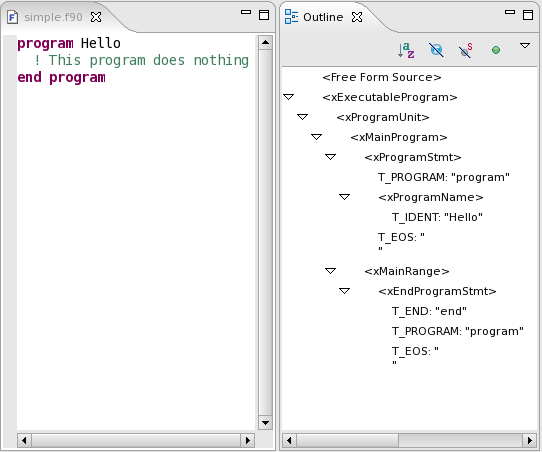
\includegraphics[width=5in]{images/parsetree1.png}
\caption{Sample program and its parse tree}
\label{parsetree}
\end{figure}

Figure \ref{parsetree} shows a trivial program and its parse tree.

\begin{itemize}

\item The node labels in angle brackets, such as $<$xExecutableProgram$>$ and
$<$xProgramStmt$>$, are nonterminals in the grammar and correspond to
\texttt{ParseTreeNodes} in the parse tree.\footnote{Note that $<$Free Form
Source$>$ (at the top of the Outline view) is just a label and not part of
the parse tree.}

\item Terminals in the grammar have names starting with T\_: for example,
T\_PROGRAM is the ``program'' keyword and T\_IDENT is an identifier.
Notice that the carriage return is also a token: end-of-statement (T\_EOS).
In the figure, these identify \texttt{Token}s in the parse
tree.\footnote{The distinction between terminals and tokens is somewhat
subtle.  Terminals are things like ``identifier,'' ``plus sign,'' and
``float'' that appear in a grammar.  Tokens are the actual chunks of text
from your input file, such as ``hello,'' ``+,'' and ``3.14.''  Every token
\textit{corresponds} to a terminal, e.g., ``hello'' is an identifier,
``+'' is (the only representation of) a plus sign, and ``3.14'' is a
float.}

\end{itemize}

Recall that each parse tree node corresponds to a nonterminal (on the
left-hand side of a production in the grammar) and each token corresponds
to a terminal.  

You can determine the nonterminal corresponding to a \texttt{ParseTreeNode}
by invoking \texttt{ParseTreeNode\#getRootNonterminal}.  (This method name
will soon be changed to \texttt{getCorrespondingNonterminal} or something
more intuitive like that.)  This will return a \texttt{Nonterminal}.  The
only valid \texttt{Nonterminal}s are all constants in the \texttt{Nonterminal}
class, so you can do identity comparisons like this:
\begin{verbatim}
if (parseTreeNode.getRootNonterminal() == Nonterminal.XEXECUTABLEPROGRAM) ...
\end{verbatim}

Similarly, you can determine the terminal corresponding to a token by
calling \texttt{Token\#getTerminal} and doing an identity comparison, as in
\begin{verbatim}
if (token.getTerminal() == Terminal.T_IDENT) ...
\end{verbatim}
You can get the text of the token (``Hello'' for the only T\_IDENT in
Figure \ref{parsetree}) by calling \texttt{Token\#getText}.

\texttt{Terminal}s and \texttt{Nonterminal}s both have a
\texttt{getDescription} method which returns a (String) description of that
terminal or nonterminal, e.g., ``T\_IDENT'' or ``$<$xExecutableProgram$>$.''
